\chapter{可测函数}

本章先给出可测空间、测度空间的概念, 首先
\[
\mbox{空间~} = \mbox{~集合~} + \mbox{~一定结构或运算}
\]
例如, 定义了线性运算的集合~$(X,\,+,\cdot)$, 称为线性空间\index{线性空间};\
定义了距离的集合~$(X,\,d)$, 称为距离空间\index{距离空间}.

\begin{example}
设~$X$~为非空集, $\T$~是~$X$~的子集族, 且满足

(i) $\emptyset, \, X \in \T$;

(ii) 若~$A_1,\,\cdots,\,A_m \in \T$, 则~$\smallcap\limits_{k=1}^m A_k \in \T$;

(iii) 若~$A_1,\,A_2,\,\cdots \in \T$, 则~$\smallcup\limits_{k=1}^\infty A_k \in \T$.

\noindent 则称~$\T$~是~$X$~上的一个拓扑, $\T$~中的元称为开集, $(X,\,\T)$~
称为拓扑空间\index{拓扑空间}.
\end{example}

\begin{definition}
设~$X$~为非空集, 若~$X$~的子集族~$\F$~是~$\sigma$-代数, 即:

(i) $\emptyset \in \F$;

(ii) 若~$A \in \F$, 则~$A^c \in \F$;

(iii) 若~$A_n \in \F, \, n = 1,\,2,\,\cdots$, 则~$\smallcup
\limits_{n = 1}^\infty A_n \in \F$.

\noindent 若~$\F$~为~$\sigma$-代数，则可以对~$\F$~中的元定义测度, $\F$~中的元称为~$\F$-可测集,
简称可测集. 此时, 称二元组~$(X,\,\F)$~为可测空间\index{可测空间}.
\end{definition}

\begin{definition}
设~$(X,\,\F)$~为可测空间, 在~$\F$~上定义测度记为~$\mu$, 则称三元组
~$(X,\,\F,\,\mu)$~为测度空间\index{测度空间}.
\end{definition}

通常用~$(\R^n,\,\F,\,\mu)$~表示勒贝格测度空间, 其中~$\F$~为
~$\R^n$~中的勒贝格可测集, $\mu$~表示勒贝格测度.

定义在测度空间上的函数可以自然产生出各种各样的集合. 为用测度论的方法研究这个函数, 特别是在定义勒贝格积分时, 必须要求这些集合是勒贝格可测集, 由此产生了可测函数的概念. 勒贝格可积函数首先必须是可测函数. 本章介绍可测函数的定义、性质及构造, 可测函数的几种收敛性以及著名的叶戈洛夫定理、卢津定理、里斯定理.

\section{可测函数及其性质}

\subsection{可测函数的概念}

\begin{definition}
设~$E$~为可测集, $f: \: E \to \R \cup \{\pm \infty\}$~为实值函数, 若对~$\forall~a \in \R$, 都有~$\{x \in E: \: f(x) > a\}$~是可测集, 则称~$f$~为可测函数
\footnote{设~$f$~为波雷尔集~$E$~上的实值函数, 若对~$\forall~a \in \R$, 都有~$\{x \in E: \: f(x) > a\}$~是波雷尔集, 则称~$f(x)$~为~$E$~上的波雷尔可测函数\index{波雷尔可测函数}.}\index{可测函数}.
\end{definition}

\begin{definition}[用可测空间描述可测函数]
设~$(X,\,\F)$~为可测空间, $E$~为可测集, $f: \: E \to \R \cup \{\pm \infty\}$~为实值函数, 若对~$\forall~a \in \R$, 都有~$\{x \in E: \: f(x) > a\} \in \F$, 则称~$f$~为~$\F$-可测函数.
\end{definition}

\begin{proposition}[可测函数的等价定义] \label{prop311}
\quad ~~~(i) $f$~可测;\

$\Leftrightarrow$ ~ (ii) ~$\forall~a \in \R,\,\{x \in E: \: f(x) \geqslant a\}$~是可测集;\

$\Leftrightarrow$ ~ (iii) ~$\forall~a \in \R,\,\{x \in E: \: f(x) < a\}$~是可测集;\

$\Leftrightarrow$ ~ (iv) ~$\forall~a \in \R,\,\{x \in E: \: f(x) \leqslant a\}$~是可测集;\

$\Rightarrow$ ~ (v) ~$\forall~a,\,b \in \R,\, a < b, \,\{x \in E: \: f(x) \in [a,\,b) \}$~是可测集.

若~$|f(x)| < +\infty$, 则~(i)-(v)~等价.
\end{proposition}

\begin{proof}
(i) $\Rightarrow$ (ii). $f$~可测, 则~$\forall~a \in \R, \, \{x \in E: \: f(x) > a\}$~是可测集, 故
\[
\{x \in E: \: f(x) \geqslant a\} = \medcap_{n=1}^\infty \Big\{x \in E: \: f(x) > a - \frac{1}{n} \Big\}
\]
是可测集.

(ii) $\Rightarrow$ (iii). $\{x \in E: \: f(x) < a\} = \{x \in E: \: f(x) \geqslant a\}^c$~可测.

(iii) $\Rightarrow$ (iv). $\{x \in E: \: f(x) \leqslant a\} = \bigcap\limits_{n=1}^\infty \{x \in E: \: f(x) < a + 1/n\}$~可测.

(iv) $\Rightarrow$ (i).  $\{x \in E: \: f(x) > a\} = \{x \in E: \: f(x) \leqslant a\}^c$~可测. 故~(i)-(iv)~等价.

$\Rightarrow$ (v). 由~(ii)~和~(iii)~得
\[
\{x \in E: \: a \leqslant f(x) < b\} = \{x \in E: \: f(x) \geqslant a\} \cap \{x \in E: \: f(x) < b\}
\]
是可测集.

若~$|f(x)| < +\infty$, 则~$\{x \in E: \: f(x) = + \infty\} = \emptyset$, 从而
\[
\{x \in E: \: f(x) \geqslant a\} = \medcup\limits_{n=1}^\infty \{x \in E: \: a \leqslant f(x) < n\} \cup \{x \in E: \: f(x) = + \infty\}
\]
是可测集.
\end{proof}

\begin{remark}
条件~(v)~中的``~$[a,\,b)$''~换成~$\R$~中任一波雷尔集, 结论仍成立.
\end{remark}

\begin{proposition}
设~$f$~可测, 则下列集合都是可测集
\[
\{x \in E: \: f(x) = a\}, \quad \{x \in E: \: f(x) < +\infty \}
\]
\[
\{x \in E: \: f(x) > -\infty \}, \quad \{x \in E: \: |f(x)| = +\infty \}
\]
\end{proposition}

\begin{proof}
利用命题~\ref{prop311}, 只需注意到下述事实
\[
\{x \in E: \: f(x) = a\} = \{x \in E: \: f(x) \leqslant a\} \cap \{x \in E: \: f(x) \geqslant a\}
\]
\[
\{x \in E: \: f(x) < +\infty\} = \medcup_{n=1}^\infty \big\{x \in E: \: f(x) < n\big\}
\]
\[
\{x \in E: \: f(x) > -\infty\} = \medcup_{n=1}^\infty \big\{x \in E: \: f(x) > -n \big\}
\]
\[
\{x \in E: \: |f(x)| = +\infty\} = \medcap_{n=1}^\infty \big\{x \in E: \: |f(x)| \geqslant n\big\}
\]
\end{proof}

\begin{example} \label{ex311}
由于零测集的任意子集都是零测集(可测), 故定义在零测集上的任何函数都是可测函数.
\end{example}

\begin{definition}
设~$E = \smallcup\limits_{i=1}^n E_i$, $E_i$~可测且互不相交, 若定义在~$E$~上的函数
~$f(x)$~在每个~$E_i$~上取常数值~$c_i$, 即~$f(x) = \sum\limits_{i=1}^n c_i \chi_{E_i} (x)$, 则称~$f(x)$~是~$E$~上的简单函数\index{简单函数}.
\end{definition}

\begin{example} \label{ex312}
简单函数是可测函数.
\end{example}

\begin{proof}
不妨设~$c_1 < c_2 < \cdots < c_n$, 对~$\forall~a \in \R$, 有
\[
\{x \in E: \: f(x) > a\} = \left\{\!\!
\begin{array}{cl}
\emptyset, & \quad \mbox{若~} a \geqslant c_n \\
E_n, & \quad \mbox{若~} c_{n-1} \leqslant a < c_n \\
E_n \cup E_{n-1}, & \quad \mbox{若~} c_{n-2} \leqslant a < c_{n-1} \\
\vdots & \qquad  \qquad \vdots \\
E_n \cup \cdots \cup E_2,  & \quad \mbox{若~} c_1 \leqslant a < c_2 \\
E, & \quad \mbox{若~} a < c_1
\end{array}
\right.
\]
均是可测集, 故~$f(x)$~可测.
\end{proof}

\begin{example}
狄利克雷函数
\[
D(x) = \left\{ \!\!
\begin{array}{ll}
1, & x \mbox{~为~} [0,\,1] \mbox{~上的有理数~} \\[0.1cm]
0, & x \mbox{~为~} [0,\,1] \mbox{~上的无理数~}
\end{array}
\right.
\]
是可测函数.
\end{example}

\begin{proof}
对~$\forall~a \in \R$, 有
\[
\{x \in [0,\,1]: \: D(x) > a\} = \left\{\!\!
\begin{array}{cl}
\emptyset, & \quad \mbox{若~} a \geqslant 1 \\[0.1cm]
\Q_{[0,1]}, & \quad \mbox{若~} 0 \leqslant a < 1 \\[0.1cm]
{[}0,\,1{]}, & \quad \mbox{若~} a < 0
\end{array}
\right.
\]
均是可测集, 故~$D(x)$~可测.
\end{proof}

\begin{example}
连续函数是可测函数.
\end{example}

\begin{proof}
设~$f$~是定义在可测集~$E$~上的连续函数, 对~$\forall~a \in \R$, 记~$E_a = \{x \in E: \: f(x) > a\}$, 下面证明~$E_a$~是可测集.

任取~$x_0 \in E_a$, 则~$f(x_0) > a$. 令~$\varepsilon = f(x_0) - a > 0$, 由~$f$~连续, 则~$\exists~\delta > 0$~使得, 当~$x \in U(x_0,\,\delta) \cap E$~时, 有
\[
a = f(x_0) - \varepsilon < f(x) < f(x_0) + \varepsilon
\]
故~$U(x_0,\,\delta) \cap E \subset E_a$. 令~$G = \smallcup\limits_{x \in E_a} U(x,\,\delta_x)$, 则~$G$~是开集, 且
\[
G \cap E = \big( \medcup_{x \in E_a} U(x,\,\delta_x) \big) \cap E = \medcup_{x \in E_a} \big( U(x,\,\delta_x) \cap E \big) \subset E_a
\]
\[
E_a \subset \big( \medcup_{x \in E_a} U(x,\,\delta_x) \big) \cap E = G \cap E
\]
故~$G \cap E = E_a$, 再由~$G \cap E$~是可测集, 故~$E_a$~是可测集.
\end{proof}

\begin{example}
单调函数是可测函数.
\end{example}

\begin{proof}
不妨设~$f$~是定义在可测集~$E$~上的单调递增函数, 记~$R(f)$~表示~$f$~的值域.
对~$\forall~a \in \R$, 有
\[
\{x \in E: \: f(x) \geqslant a\} = \left\{\!\!
\begin{array}{cl}
\emptyset & \quad \mbox{若对~}\forall~ y \in R(f), \, \mbox{都有~} a > y \\[0.1cm]
E, & \quad \mbox{若对~}\forall~ y \in R(f), \, \mbox{都有~} a < y \\[0.1cm]
{[}x_0,\,+\infty) \cap E, & \quad \mbox{若~} a \in R(f)
\end{array}
\right.
\]
(其中, $x_0 \in E$~满足~$f(x_0) = a$)~均是可测集, 故~$f(x)$~可测.
\end{proof}

\subsection{可测函数的性质}

\begin{definition}
若~$m\{x \in E: \: f(x) \neq g(x)\} = 0$, 则称函数~$f$~与~$g$~在~$E$~上几乎处处\index{几乎处处}相等, 也称~$f$~与~$g$~对等. 记为~$f(x) = g(x), \, \mathrm{a.e.~} x \in E$.

若~$m\{x \in E: \: |f(x)| = + \infty\} = 0$, 则称函数~$f$~在~$E$~上几乎处处有限.

若~$f(x) = 0, \, \mathrm{~a.e.~} x \in E$, 则称~$f(x)$~为~$E$~上的零函数\index{零函数}.
\end{definition}

\begin{proposition} \label{prop313}
(i) 设~$f(x)$~在~$E$~上可测, $E_0$~是~$E$~的可测子集, 则~$f|_{E_0}(x)$;

(ii) 设~$f(x)$~在~$E_k$~上可测, $E = \smallcup\limits_k E_k$, 则~$f(x)$~在~$E$~上可测.
\end{proposition}

\begin{proof}
(i) $\{x \in E_0: \: f(x) > a\} = \{x \in E: \: f(x) > a\} \cap E_0$.

(ii) $\{x \in E: \: f(x) > a\} = \smallcup\limits_k\{x \in E_k: \: f(x) > a\}$.
\end{proof}

\begin{proposition}
若~$f(x)$~在~$E$~上可测, $g(x) = f(x), \, \mathrm{a.e.~} x \in E$, 则~$g(x)$~在~$E$~上可测.
\end{proposition}

\begin{proof}
令
\[
E_1 = \{x \in E: \: g(x) = f(x)\}, \quad E_2 = \{x \in E: \: g(x) \neq f(x)\}
\]
则~$E = E_1 \cup E_2$~且~$m(E_2) = 0$, 从而$E_1$可测. 由命题~\ref{prop313}~(i), $g|_{E_1} = f|_{E_1}$~可测; 由本节的例~\ref{ex311}, $g|_{E_2}$~可测, 再由命题~\ref{prop313}~(ii), $g$~在~$E$~上可测.
\end{proof}

\begin{definition}
设~$f(x)$~为定义在~$E$~上的函数, 则
\[
f^+(x) = \max\{f(x),\,0\} = \left\{\!\!
\begin{array}{cl}
f(x), & f(x) \geqslant 0 \\[0.1cm]
0, & f(x) < 0
\end{array}
\right.
\]
\[
f^-(x) = \max\{-f(x),\, 0\} = \left\{\!\!
\begin{array}{cl}
0, & f(x) \geqslant 0 \\[0.1cm]
-f(x), & f(x) < 0
\end{array}
\right.
\]
分别称为~$f$~的正部\index{函数正部}和负部\index{函数负部}. 
\end{definition}

显然有~$f^+(x), \, f^-(x)$~均非负, 且
\[
|f(x)| = f^+(x) + f^-(x), \quad f(x) = f^+(x) - f^-(x).
\]

\begin{figure}[!htb]
\centering
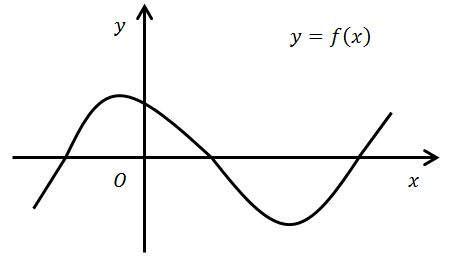
\includegraphics[width=0.31\textwidth]{image/yuanhanshu.jpg}
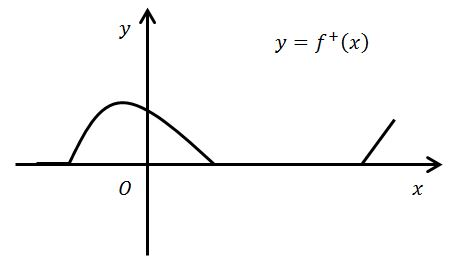
\includegraphics[width=0.31\textwidth]{image/hanshuzhengbu.jpg}
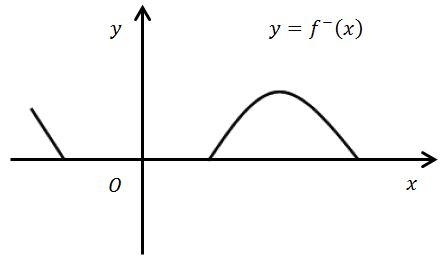
\includegraphics[width=0.31\textwidth]{image/hanshufubu.jpg}
\caption{~函数的正部与负部} \label{fig31}
\end{figure}

\begin{proposition}
设~$f(x),\,g(x)$~在~$E$~上可测, 则

(i) $f(x) \pm g(x), \, f(x)g(x), \, f(x)/g(x)$~均在~$E$~上可测;

(ii) $\max\{f(x),\,g(x)\}, \, \min\{f(x),\,g(x)\}$~均在~$E$~上可测;

(iii) $f^+(x), \, f^-(x), \, |f(x)|$~均在~$E$~上可测.
\end{proposition}

\begin{proof}
为了简单, 将~$\{x \in E: \: f(x) > a\}$~简记为~$E_{[f>a]}$.

(i) 对~$\forall~a \in \R$, 有~$E_{[f+g>a]} = E_{[f>a-g]}$. 任取~$x \in E_{[f>a-g]}$, 则~$f(x) > a - g(x)$. 由于有理数集~$\Q$~可列且在
~$\R$~中稠密, 则~$\exists~r_0 \in \Q$~使得
\[
f(x) > r_0 > a - g(x)
\]
故~$x \in E_{[f>r_0]}$~且~$x \in E_{[g>a-r_0]}$, 从而
\[
x \in \medcup\limits_{r \in \Q} \big( E_{[f>r]} \cap E_{[g>a-r]}\big)
\]
于是
\[
E_{[f>a-g]} \subset \medcup\limits_{r \in \Q} \big( E_{[f>r]} \cap E_{[g>a-r]}\big)
\]

反过来, 若存在~$r_0 \in \Q$~使得~$x \in  E_{[f>r_0]} \cap E_{[g>a-r_0]}$, 则
\[
f(x) > r_0, \quad g(x) > a - r_0
\]
故~$f(x) > r_0 > a - g(x)$, 从而~$x \in E_{[f>a-g]}$. 因此
\[
E_{[f>a-g]} =\medcup\limits_{r \in \Q} \big( E_{[f>r]} \cap E_{[g>a-r]}\big)
\]
$f,\,g$~可测保证上式右端是可测集, 从而~$f(x)+g(x)$~可测.

类似可证~$f(x)-g(x)$~可测.

先证~$f^2(x)$~可测. 由于
\[
E_{[f^2>a]} = \left\{
\begin{array}{cl}
E, & \quad \mbox{若~} a < 0 \\[0.1cm]
E_{[f>\sqrt{a}]} \cup E_{[f<-\sqrt{a}]}, & \quad \mbox{若~} a \geqslant 0
\end{array}
\right.
\]
是可测集, 故~$f^2(x)$~可测.

注意到
\[
f(x)g(x) = \frac{1}{4} \cdot \big[ \big( f(x) + g(x) \big)^2 - \big( f(x) - g(x) \big)^2 \big]
\]
故~$f(x)g(x)$~可测.

先证~$1/g(x)$~可测. 由于
\begin{eqnarray*}
E_{[1/g>a]} &=& E_{[g>0,g<1/a]} \medcup E_{[g<0,g>1/a]} \\
&=& \big(E_{[g>0]} \medcap E_{[g<1/a]} \big) \medcup \big(E_{[g<0]} \medcap E_{[g>1/a]} \big)
\end{eqnarray*}
是可测集, 故~$1/g(x)$~可测. 从而~$f(x)/g(x) = f(x)\cdot\big(1/g(x)\big)$~可测.

(ii) 由于
\[
E_{[\max\{f,g\}>a]} = E_{[f>a]} \medcup E_{[g>a]}, \quad E_{[\min\{f,g\}>a]} = E_{[f>a]} \medcap E_{[g>a]}
\]
故~$\max\{f(x),\,g(x)\}, \, \min\{f(x),\,g(x)\}$~可测.

(iii) 由~(ii)~以及~$f^+(x), \, f^-(x)$~的定义知, $f^+(x),\,f^-(x)$~可测. 再由~$|f(x)| = f^+(x) + f^-(x)$~及~(i)~知, $|f(x)|$~可测.
\end{proof}

\begin{proposition} \label{prop316}
设~$f_n(x), \, n = 1,\,2,\,\cdots$~在~$E$~上可测, 则
\[
\sup_n f_n(x),\quad \inf_n f_n(x),\quad \limsup_{n \to \infty} f_n(x), \quad \liminf_{n \to \infty} f_n(x), \quad \lim_{n \to \infty} f_n(x)
\]
均在~$E$~上可测.
\end{proposition}

\begin{proof}
由于
\[
\{x \in E: \: \sup_n f_n(x) > a\} = \medcup_{n=1}^\infty \{x \in E: \: f_n(x) > a\}
\]
\[
\{x \in E: \: \inf_n f_n(x) > a\} = \medcap_{n=1}^\infty \{x \in E: \: f_n(x) > a\}
\]
故~$\sup\limits_n f_n(x),\, \inf\limits_n f_n(x)$~可测. 又
\[
\limsup_{n \to \infty} f_n(x) = \inf_{k \geqslant 1} \big( \sup_{n \geqslant k}f_n(x) \big)
\]
故~$\limsup\limits_{n \to \infty} f_n(x)$~可测. 再由
\[
\liminf_{n \to \infty} f_n(x) = -\limsup_{n \to \infty} \big( -f_n(x) \big)
\]
故~$\liminf\limits_{n \to \infty} f_n(x)$~可测.

最后, 若~$\lim\limits_{n \to \infty} f_n(x)$~存在, 则
\[
\lim_{n \to \infty} f_n(x) = \limsup_{n \to \infty} f_n(x) = \liminf_{n \to \infty} f_n(x)
\]
也可测.
\end{proof}

\begin{remark}
我们知道, 连续函数的极限不一定是连续函数, 但由命题~\ref{prop316}, 可测函数的极限是可测函数, 这为处理一些问题带来极大的方便.
\end{remark}

\begin{proposition}
在~$\R$~上, 若~$g$~连续, $f$~可测, 则~$g \circ f$~可测.
\end{proposition}

\begin{proof}
对~$\forall~a \in \R$, 有
\[
\{x \in E: (g \circ f) (x) > a\} = (g \circ f)^{-1}(a,\,+\infty) = f^{-1} \big( g^{-1} (a,\, +\infty) \big)
\]
由于~$g$~连续, 故~$g^{-1} (a,\, +\infty)$~是开集, 记~$g^{-1} (a,\, +\infty) = \smallcup\limits_{k} (\alpha_k,\,\beta_k)$. 则
\begin{eqnarray*}
f^{-1} \big( g^{-1} (a,\, +\infty) \big) &=& f^{-1} \big( \medcup_{k} (\alpha_k,\,\beta_k) \big) = \medcup_{k} f^{-1} (\alpha_k,\,\beta_k) \\
&=& \medcup_{k}\{x \in E: \: \alpha_k < f(x) < \beta_k\} \\
&=& \big( \medcup_{k}\{x \in E: \: f(x) > \alpha_k \big\}) \medcap \big( \medcup_{k}\{x \in E: \: f(x) < \beta_k \big\})
\end{eqnarray*}
是可测集, 从而~$g \circ f$~可测.
\end{proof}

\begin{remark}
$f \circ g$~不一定可测, 从而两个可测函数的复合也不一定是可测函数. 绝对连续函数(\S 5.3)可将可测集映射为可测集, 然而严格单调的连续函数也不能将可测集映射为可测集
(可测函数更不能保证这一点). 例如, 设~$\varphi$~为~$[0,\,1]$~上的康托尔函数, 令
\[
h(x) = \frac{x + \varphi(x)}{2}
\]
则~$h: [0,\,1] \rightarrow [0,\,1]$~为严格递增的连续函数, 且~$m\big(h(C)\big)=1/2$, 其中~$C$~为康托尔集.
取~$W \subset h(C)$~为不可测集, 则~$M = h^{-1}(W)$~可测, 而~$h(M) = W$~不可测.

连续映射能保证波雷尔集的原象是波雷尔集, 但不能保证可测集的原象仍为可测集(可测函数更不能保证这一点). 例如, 前面的函数~$h$~为~$[0,\,1]$~到~$[0,\,1]$~的同胚映射\footnote{$h$~为一一映射, 且~$h$~与~$h^{-1}$~均连续.}, 易知其反函数~$h^{-1}$~在~$[0,\,1]$~也是严格递增的连续函数, 且可测集~$M$~在~$h^{-1}$~的原象~$W$~是不可测集.

进一步, 若记~$g = h^{-1}$~连续且严格递增, $W$~不可测, $g(W) = M$~可测. 令
\[
f = \chi_M(x), \quad x \in [0,\,1]
\]
则~$f$~可测. 由于
\[
\big\{ x \in [0,\,1]: \: f\big(g(x)\big) \neq 0 \big\} = \big\{ x \in [0,\,1]: \: g(x) \in M \big\} = W
\]
不可测, 故复合函数~$(f \circ g) = f\big(g(x)\big)$~不可测.
\end{remark}

\subsection{可测函数的构造}

简单函数只在有限个可测子集上取有限个实值, 从结构上来看是最简单的一类可测函数. 下面的定理将给出简单函数与一般可测函数的联系, 本书后面许多重要结果都是基于此得到的.

\begin{theorem}[可测函数构造定理\index{可测函数构造定理}] \label{thm311}
设~$f(x)$~为~$E$~上的非负可测函数, 则存在一列递增的非负简单函数~$\{ \varphi_n(x) \}$~满足~$\varphi_n \to f$(处处收敛),  即
\[
f(x) = \lim_{n \to \infty} \varphi_n(x), \quad \forall x \in E
\]
若~$f$~有界, 则~$\varphi_n \rightrightarrows f$(一致收敛).
\end{theorem}

\begin{proof}
(对值域做划分)对每个~$n \in \N$, 把~$[0,\,n]$~分为~$n^2$~等份, 即每段的长度是~$1/n$, 记
\[
E_{n,k} = \Big\{ x \in E: \: \frac{k-1}{n} \leqslant f(x) < \frac{k}{n} \Big\}, \quad k=1,\,\cdots,\, n^2
\]
\[
E_n = \{ x \in E: \: f(x) \geqslant n\}
\]

\begin{figure}[!htb]
\centering
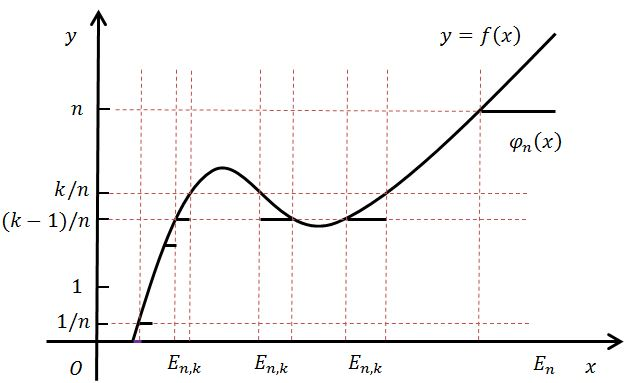
\includegraphics[width=0.8\textwidth]{image/kecehanshugouzao.jpg}
\vspace*{-0.2cm}
\caption{~可测函数的构造} \label{fig32} 
\end{figure}

注意到~$f$~在~$E$~上非负, 则有~$\big( \smallcup\limits_{k=1}^{n^2} E_{n,k} \big) \smallcup E_n = E$. 对~$\forall~x \in E$, 令
\[
\begin{array}{ll}
\varphi_n(x) = \left\{\!\!
\begin{array}{cl}
\dfrac{k-1}{n}, & x \in E_{n,k} \\[0.1cm]
n, & x \in E_n
\end{array}
\right.

\end{array}
\]
其中~$k = 1, \, \cdots, \, n^2$. 即
\[
\varphi_n(x) = \sum_{k=1}^{n^2} \frac{k-1}{n} \chi_{E_{n,k}}(x) + n \chi_{E_n}(x), \quad x \in E
\]

显然, $\varphi_n(x)$~是非负简单函数, 且
\[
\varphi_n(x) \leqslant \varphi_{n+1}(x) \leqslant f(x), \, \varphi_n(x) \leqslant n
\]
于是, 对~$\forall~x \in E$, 若~$f(x) < +\infty$, 则当~$n \geqslant f(x)$~时, 有
\[
0 \leqslant f(x) - \varphi_n(x) < \frac{1}{n}
\]
令~$n \to \infty$~得~$\lim\limits_{n \to \infty} \varphi_n(x) = f(x)$. 若~$f(x) = +\infty$, 则~$\varphi_n(x) = n, \, \forall~n \in \N$, 也有~$\lim\limits_{n \to \infty} \varphi_n(x) = f(x)$.

若~$f$~有界, 则存在~$M > 0$, 使得~$f(x) \leqslant M, \, \forall~x \in E$. 从而当~$n > M$~时, 有
\[
\sup_{x \in E} |f(x) - \varphi_n(x)| \leqslant \frac{1}{n}
\]
故~$\varphi_n \rightrightarrows f$.
\end{proof}

\begin{theorem} \label{thm312}
设~$f(x)$~为~$E$~上的可测函数, 则存在简单函数列~$\{ \varphi_n(x) \}$~满足
~$\varphi_n \to f$~且~$|\varphi_n(x)| \leqslant |f(x)|$. 若~$f$~有界, 则~$\varphi_n \rightrightarrows f$.
\end{theorem}

\begin{proof}
由于~$f(x) = f^+(x) - f^-(x)$, 则~$f^+(x),\,f^-(x)$~是非负可测函数. 由定理~\ref{thm311}, 存在简单函数列~$\{\varphi^{(1)}_n(x)\}, \{\varphi^{(2)}_n(x)\}$, 使得
\[
\lim_{n \to \infty} \varphi^{(1)}_n(x) = f^+(x), \quad \lim_{n \to \infty} \varphi^{(2)}_n(x) = f^-(x)
\]
令~$\varphi_n(x) = \varphi^{(1)}_n(x) - \varphi^{(2)}_n(x)$, 则容易验证~$\varphi_n(x)$~是简单函数, 且
\[
\lim_{n \to \infty} \varphi_n(x) = \lim_{n \to \infty} \big[\varphi^{(1)}_n(x) - \varphi^{(2)}_n(x) \big] = f^+(x) - f^-(x) = f(x)
\]
若~$f$~有界, 则~$f^+, \, f^-$~都有界, 由定理~\ref{thm311}, $\varphi^{(1)}_n \rightrightarrows f^+, \, \varphi^{(2)}_n \rightrightarrows f^-$, 从而
\[
\varphi_n = \varphi^{(1)}_n - \varphi^{(2)}_n \rightrightarrows f^+ - f^- = f
\]
定理得证.
\end{proof}

\begin{corollary}
$f$~可测~$\Leftrightarrow$~存在简单函数列~$\{ \varphi_n\}$~使得~$\varphi_n \rightarrow f$.
\end{corollary}

\begin{proof}
只需证充分性. 由于~$\varphi_n$~可测, 由命题~\ref{prop316}~知, $f(x) = \lim\limits_{n \to \infty} \varphi_n(x)$~可测.
\end{proof}

\section{可测函数列的收敛性}

可测函数列可以定义各种收敛性, 本节讨论几乎处处收敛、依测度收敛和接近一致收敛. 勒贝格定理、叶戈洛夫定理、里斯定理等揭示了几种收敛性之间的一些蕴含关系.

\subsection{几种收敛性}

\begin{definition}
设~$\{f_n(x)\}$~为~$E$~上的函数列, 对任意给定的~$x \in E$, 若对~$\forall~\varepsilon > 0$, $\exists~N_{\varepsilon,x} \in \N$, 使得当~$n \geqslant N_{\varepsilon,x}$~时, 有
\[
|f_n(x) - f(x)| < \varepsilon
\]
则称~$f_n(x)$~在~$E$~上处处收敛\index{处处收敛}\footnote{也称为点点收敛或收敛, 等价于~$\lim\limits_{n \to \infty} f_n(x) = f(x), \, \forall~x \in E$.}于~$f(x)$, 简记为~$f_n \rightarrow f$.
\end{definition}

\begin{definition}
设~$\{f_n(x)\}$~为~$E$~上的函数列, 若对~$\forall~\varepsilon > 0$,
$\exists~N_\varepsilon \in \N$, 使得当~$n \geqslant N_\varepsilon$~时, 有
\[
|f_n(x) - f(x)| < \varepsilon, \,\quad \forall~ x \in E
\]
或等价地, 若
\[
\lim_{n \to \infty} \sup_{x \in E} |f_n(x) - f(x)| = 0
\]
则称~$f_n(x)$~在~$E$~上一致收敛\index{一致收敛}于~$f(x)$, 简记为~$f_n \rightrightarrows f$.
\end{definition}

\begin{definition}
设~$\{f_n(x)\}$~为~$E$~上的函数列, 若存在零测集~$E_0 \subset E$, 使得~$f_n(x)$~在~$E - E_0$~上处处收敛于~$f(x)$, 则称~$f_n(x)$~在~$E$~上几乎处处收敛\index{几乎处处收敛}于~$f(x)$, 简记为~$f_n \xrightarrow{\mathrm{a.e.}} f$.
\end{definition}

\begin{remark}
在函数对等的意义下, 几乎处处收敛的极限函数是唯一的.
\end{remark}

\begin{proof}
设在可测集~$E$~上有~$f_n \xrightarrow{\mathrm{a.e.}} f,\, f_n \xrightarrow{\mathrm{a.e.}} g$. 则存在零测集~$E_1, \, E_2 \subset E$~使得
\[
f_n(x) \rightarrow f(x), \, \quad x \in E - E_1
\]
\[
f_n(x) \rightarrow g(x), \, \quad x \in E - E_2
\]
由于处处收敛的极限函数是唯一的, 故
\[
f(x) = g(x), \quad \forall~x \in E - (E_1 \cup E_2)
\]
注意到~$E_1 \cup E_2$~是零测集, 从而~$f(x) = g(x), \, \mathrm{~a.e.~} x \in E$.
\end{proof}

\begin{definition}
设~$\{f_n(x)\}$~为~$E$~上的函数列, 若对~$\forall~\varepsilon > 0$, 都有
\[
\lim_{n \to \infty} m\big( \{x \in E: \: |f_n(x) - f(x)| \geqslant \varepsilon\} \big) = 0
\]
或等价地,
若对~$\forall~\varepsilon > 0$~及~$\delta > 0$, 存在~$N_{\varepsilon,\delta} \in \N$, 使得当~$n \geqslant N_{\varepsilon,\delta}$~时, 有
\[
m\big( \{x \in E: \: |f_n(x) - f(x)| \geqslant \varepsilon\} \big) < \delta
\]
则称~$f_n(x)$~在~$E$~上依测度收敛\index{依测度收敛}于~$f(x)$, 简记为~$f_n \xrightarrow{~\mu~} f$.
\end{definition}

\begin{remark}
在函数对等的意义下, 依测度收敛的极限函数是唯一的.
\end{remark}

\begin{proof}
设在可测集~$E$~上有~$f_n \xrightarrow{~\mu~} f,\, f_n \xrightarrow{~\mu~} g$, 则对~$\forall k \in \N$, 有
\[
m(\{x \in E: |f_n(x) - f(x)| \geqslant \frac{1}{2k}\}) \to 0, \quad n \to +\infty
\]
\[
m(\{x \in E: |f_n(x) - g(x)| \geqslant \frac{1}{2k}\}) \to 0, \quad n \to +\infty
\]
对任意的~$n \in N$, 由于
\[
|f(x) - g(x)| \leqslant |f(x) - f_n(x)| + |f_n(x) - g(x)|
\]
故
\begin{eqnarray*}
&& \{x \in E: \: |f(x) - g(x)| \geqslant 1/k\} \\
&\subset& \Big\{x \in E: \: |f(x) - f_n(x)| \geqslant \frac{1}{2k} \Big\} \medcup \Big\{x \in E: \: |f_n(x) - g(x)| \geqslant \frac{1}{2k} \Big\}
\end{eqnarray*}
从而
\begin{eqnarray*}
	&& m(\{x \in E: \: |f(x) - g(x)| \geqslant 1/k\}) \\
	&\leqslant& m(\Big\{x \in E: \: |f(x) - f_n(x)| \geqslant \frac{1}{2k} \Big\}) + m(\Big\{x \in E: \: |f_n(x) - g(x)| \geqslant \frac{1}{2k} \Big\})
\end{eqnarray*}
令~$n \to \infty$, 可得~$m(\{x \in E: \: |f(x) - g(x)| \geqslant 1/k\})=0, \, \forall k \in \N$. 又
\[
\{x \in E: \: f(x) \neq g(x)\} = \medcup_{k=1}^\infty\{ x \in E: \: |f(x) - g(x)| \geqslant 1/k \}
\]
故
\[
m\big(\{x \in E: \: f(x) \neq g(x)\}\big) \leqslant \sum_{k=1}^\infty m(\{x \in E: \: |f(x) - g(x)| \geqslant 1/k\}) = 0
\]
因此，$f(x) = g(x), \, \mathrm{a.e.~} x \in E$.
\end{proof}

四种收敛间的关系: (前三个蕴含显然, 后一个蕴含见命题~\ref{prop321})
\[
f_n \rightrightarrows f ~ \Longrightarrow ~ f_n \rightarrow f ~ \Longrightarrow ~ f_n \xrightarrow{\mathrm{a.e.}} f \xLongrightarrow{m(E)<+\infty} f_n \xrightarrow{~\mu~} f
\]

\begin{example}[收敛但不一致收敛]
$f_n(x) = x^n, \, n=1,\,2,\,\cdots$~在~$[0,\,1]$~上处处收敛于
\[
f(x) = \left\{\!\!
\begin{array}{ll}
0, &  0 \leqslant x < 1 \\
1, &  x = 1
\end{array}
\right.
\]
但不一致收敛于~$f(x)$, 因为连续函数列的一致收敛极限必连续, 而~$f(x)$~不连续. 然而, 去掉任意小的一段之后
一致收敛, 即: 对~$\forall~\delta > 0$, $f_n(x)$~在~$[0,\,1-\delta]$~上一致收敛于~$0$.
\end{example}

\begin{example}[依测度收敛但不几乎处处收敛]
对每个~$n \in \N$, 都存在唯一的~$k,\,i \in \N$, 使得
\[
n = 2^k + i, \quad 0 \leqslant i < 2^k
\]
定义~$[0,\,1]$~上的函数
\[
f_n(x) = \chi_{[\frac{i}{2^k},\frac{i+1}{2^k})} (x), \quad n = 1,\,2,\,\cdots
\]
任取~$x_0 \in [0,\,1]$, 对每个~$k \in \N$, $\exists~0 \leqslant i_k < 2^k$~使得
\[
x_0 \in \big[\frac{i_k}{2^k},\frac{i_k+1}{2^k}\big)
\]
记~$n_k = 2^k + i_k$, 则
\[
f_{n_k}(x_0) = 1, \quad k = 1,\, 2,\,\cdots
\]
可见, $\{f_n(x_0)\}$~有无穷多项为~$1$, 无穷多项为~$0$. 故~$f_n(x)$~在~$[0,\,1]$~上每个点都不收敛(从而不是几乎处处收敛). 但对~$\forall~\varepsilon \in (0, \,1)$, 有
\[
m\big\{ x \in [0,\,1]: \: |f_n(x) - 0| \geqslant \varepsilon \big\} = \frac{1}{2^k} \to 0, \quad n \to \infty
\]
其中, $n = 2^k + i, \, 0 \leqslant i < 2^k$. 故~$f_n \xrightarrow{~\mu~} 0$. 这表明~$n$~越大, 出现~``~$1$''~的频率越趋于~$0$.
\end{example}

从几乎处处收敛与依测度收敛的定义来看, 几乎处处收敛是指在除去一个零测集~$E_0$~之外的每个点
~$x_0 \in E - E_0$~上, 其函数值数列~$\{f_n(x_0)\}$~都收敛;\
而依测度收敛是指函数列的不收敛点集~$\{x \in E: \: |f_n(x) - f(x)| \geqslant \varepsilon\}$~的测度是随着~$n$~的增大趋于~$0$~的.

\subsection{叶戈洛夫定理}

\begin{lemma} \label{lem321}
设~$\{f_n(x)\}$~为~$E$~上几乎处处有限的可测函数列, 且~$m(E) < +\infty$, 若~$f_n \xrightarrow{\mathrm{a.e.}} f$, 对~$\forall~\varepsilon > 0$, 令
\[
E_n(\varepsilon) = \big\{ x \in E: \: |f_n(x) - f(x)| \geqslant \varepsilon \big\}
\]
则有
\[
\lim_{N \to \infty} m \Big( \medcup_{n=N}^\infty E_n(\varepsilon) \Big) = 0
\]
\end{lemma}

\begin{proof}
由第一章~\S1.1~例~\ref{ex112}~的证明知, 对任意给定的~$\varepsilon > 0$, 上限集~$\mathop{\cap}\limits_{N=1}^\infty \mathop{\cup}\limits_{n = N}^\infty E_n(\varepsilon)$~中的点一定是不收敛点. 由于~$f_n \xrightarrow{\mathrm{a.e.}} f$, 故
~$m\big( \mathop{\cap}\limits_{N=1}^\infty \mathop{\cup}\limits_{n = N}^\infty E_n(\varepsilon) \big) = 0$. 注意到~$\big\{ \mathop{\cup}\limits_{n = N}^\infty E_n(\varepsilon) \big\}^\infty_{N=1}$~是单调递减集列, 由单调可测集列测度的极限性质可得
\[
\lim_{N \to \infty} m \big( \medcup_{n=N}^\infty E_n(\varepsilon) \big) =  m \big( \lim_{N \to \infty} \medcup_{n=N}^\infty E_n(\varepsilon) \big)= m\big( \medcap\limits_{N=1}^\infty \medcup\limits_{n = N}^\infty E_n(\varepsilon) \big) = 0
\]
引理证毕.
\end{proof}

\begin{theorem}[勒贝格定理\index{勒贝格定理}] \label{prop321}
设~$\{f_n(x)\}$~为~$E$~上几乎处处有限的可测函数列, 且~$m(E) < +\infty$, 若~$f_n \xrightarrow{\mathrm{a.e.}} f$, 则~$f_n \xrightarrow{~\mu~} f$.
\end{theorem}

\begin{proof}
由引理~\ref{lem321}, 对~$\forall~\varepsilon > 0$, 有
\[
\lim_{N \to \infty} m \big( \mathop{\cup}_{n=N}^\infty \big\{ x \in E: \: |f_n(x) - f(x)| \geqslant \varepsilon \big\} \big) = 0
\]
故由测度的单调性得
\begin{eqnarray*}
&& \lim_{n \to \infty} m\big( \{x \in E: \: |f_n(x) - f(x)| \geqslant \varepsilon \}\big) \\
&\leqslant& \lim_{n \to \infty} m \big( \mathop{\cup}_{k=n}^\infty \big\{ x \in E: \: |f_k(x) - f(x)| \geqslant \varepsilon \big\} \big) = 0
\end{eqnarray*}
从而, $f_n \xrightarrow{~\mu~} f$.
\end{proof}

\begin{remark}
勒贝格定理中条件~$m(E)< +\infty$~不能去掉. 例如, 取~$E = (0,\,+\infty)$, 令~$f_n(x) = \chi_{(0,n]}(x)$,
则
\[
f_n(x) \rightarrow f(x) \equiv 1, \quad x \in E
\]
但当取~$\delta = 1/2 >0$~时, 有
\[
m\big( \{x \in E: \: |f_n(x)-f(x)| \geqslant \delta\}\big) = m\big( (n,\, +\infty) \big) = +\infty
\]
故~$f_n$~不依测度收敛到~$f$.
\end{remark}

\begin{theorem}[叶戈洛夫定理\index{叶戈洛夫定理}]
设~$f_n(x),\,f(x)$~为~$E$~上几乎处处有限的可测函数, 且~$m(E) < +\infty$, 若~$f_n \xrightarrow{\mathrm{a.e.}} f$, 则对~$\forall~\delta > 0$, 存在~$E_\delta \subset E, \, m(E_\delta) < \delta$, 使得~$f_n(x)$~在~$E-E_\delta$~上一致收敛于~$f(x)$\footnote{也称~$f_n(x)$~在~$E$~上接近一致收敛于~$f(x)$.}.
\end{theorem}

\begin{proof}
由引理~\ref{lem321}, 对~$\forall~\varepsilon > 0$, 有
\[
\lim_{N \to \infty} m \big( \medcup_{n=N}^\infty E_n(\varepsilon) \big) = 0
\]
则对~$\forall~\delta > 0$, 以及每个~$k \in \N$, 都存在~$N_k$~使得
\[
m\Big( \medcup_{n = N_k}^\infty E_n\big( \frac{1}{k} \big) \Big) < \frac{\delta}{2^k}
\]
令~$E_\delta = \smallcup\limits_{k=1}^\infty \smallcup\limits_{n=N_k}^\infty E_n(1/k)$, 则
\[
m(E_\delta) \leqslant \sum_{k=1}^\infty m\Big( \medcup_{n=N_k}^\infty E_n\big( \frac{1}{k} \big) \Big) < \sum_{k=1}^\infty \frac{\delta}{2^k} = \delta
\]
下面证明~$f_n(x)$~在~$E - E_\delta$~上一致收敛于~$f(x)$. 注意到
\begin{eqnarray*}
E - E_\delta &=& E \cap E^c_\delta = E \cap \medcap\limits_{k=1}^\infty \medcap\limits_{n=N_k}^\infty E^c_n\Big( \frac{1}{k} \Big) \\
&=& \medcap\limits_{k=1}^\infty \medcap\limits_{n=N_k}^\infty \Big\{ x \in E: \: |f_n(x) - f(x)| < \frac{1}{k} \Big\}
\end{eqnarray*}
故只要~$x \in E - E_\delta$, 则对每一个~$k \in \N$, 都有
\[
x \in \medcap_{n=N_{k}}^\infty \Big\{ x \in E: \: |f_n(x) - f(x)| < \frac{1}{k} \Big\}
\]
于是, 对~$\forall~\varepsilon > 0$, 特别地, 取~$k_0 \in \N$~使得~$1/k_0 < \varepsilon$, 则
\[
x \in \medcap_{n=N_{k_0}}^\infty \Big\{ x \in E: \: |f_n(x) - f(x)| < \frac{1}{k_0} \Big\}
\]
即当~$n \geqslant N_{k_0}$~时, 有
\[
|f_n(x) - f(x)| < \frac{1}{k_0} < \varepsilon
\]
这说明~$f_n(x) \rightrightarrows f(x), \, \forall~x \in E - E_\delta$.
\end{proof}

\begin{remark}
(i) 条件~``~$m(E) < +\infty$''~不能少. 例如, 设~$E = (0,\,+\infty)$, 则~$m(E) = + \infty$. 作~$E$~上的函数列
\[
f_n(x) = \chi_{(0,\,n]} (x), \quad x \in E, \quad n = 1,\,2,\,\cdots
\]
则易知~$f_n(x)$~在~$E$~上处处收敛于~$1$. 但由于对~$\delta > 0$,
当~$m(E_\delta) < \delta$~时, 对每个~$n \in \N$, 都有~$(n,\,+\infty) - E_\delta \neq \emptyset$. 从而存在~$x_0 \in (n,\,+\infty) - E_\delta$, 于是~$f_n(x_0) = 0$.
因此, $f_n(x)$~在~$E - E_\delta$~上不一致收敛于~$1$.

\smallskip

(ii) 条件~``~$m(E_\delta) < \delta$''~不能加强到~``~$m(E_\delta) = 0$''.
例如
\[
f_n(x) = x^n, \quad x \in (0,\,1)
\]
则~$f_n(x)$~在~$(0,\,1)$~上处处收敛于~$0$. 但对任意的零测集~$E_0 \subset (0,\,1)$, 以及~$\forall~n \in \N$, 有~$(\left(1/2\right)^{\frac{1}{n}},\,1) - E_0 \neq \emptyset$. 取
\[
x_0 \in \Big(\left(\frac{1}{2}\right)^{\frac{1}{n}},\,1 \Big) - E_0 \subset E - E_0
\]
则~$f_n(x_0) = x^n_0 > 1/2$, 故~$f_n(x)$~在~$E - E_0$~上不一致收敛于~$0$.
\end{remark}

\begin{theorem}[叶戈洛夫定理的逆定理\index{叶戈洛夫定理的逆定理}]
设~$E$~上的可测函数列~$\{f_n(x)\}$~满足: $\forall~\delta > 0$, $\exists~E_\delta \subset E, \, m(E_\delta) < \delta$, 使得~$f_n(x)$~在~$E-E_\delta$~
上一致收敛于~$f(x)$, 则~$f_n \xrightarrow{\mathrm{a.e.}} f$.
\end{theorem}

\begin{proof}
分别取~$\delta_k = 1/k, \, k = 1,\,2,\, \cdots$, 则存在~$e_k \subset E, \, m(e_k) < 1/k$, 使得
\[
f_n(x) \rightrightarrows f(x), \quad x \in E - e_k
\]
记~$e = \smallcap\limits_{k=1}^\infty e_k$, 则
\[
m(e) \leqslant m(e_k) < \frac{1}{k}, \quad k = 1, \, 2, \, \cdots
\]
令~$k \to \infty$~得~$m(e) = 0$. 下面证明~$f_n(x)$~在~$E - e$~上处处收敛于~$f(x)$.

由于
\begin{eqnarray*}
E -e &=& E - \medcap\limits_{k=1}^\infty e_k = E \cap \Big( \medcup\limits_{k=1}^\infty e^c_k \Big) \\
&=& \medcup\limits_{k=1}^\infty (E \cap e^c_k) = \medcup\limits_{k=1}^\infty (E - e_k)
\end{eqnarray*}
故对~$\forall~x \in E - e$, 存在~$k_0 \in \N$, 使得~$x \in E - e_{k_0}$. 又~$f_n$~在~$E - e_{k_0}$~上一致收敛于~$f$, 从而处处收敛于~$f$, 于是在~$x$~处收敛.
\end{proof}

\subsection{里斯定理}

\begin{theorem}[里斯定理\index{里斯定理}] \label{Rieszth}
设~$\{f_n(x)\}$~为~$E$~上的可测函数列, 若~$f_n \xrightarrow{~\mu~} f$, 则存在子列~$\{f_{n_k}\} \subset \{f_n\}$~使得~$f_{n_k} \xrightarrow{\mathrm{a.e.}} f$.
\end{theorem}

\begin{proof}
由于~$f_n \xrightarrow{~\mu~} f$, 则对~$\forall~\varepsilon > 0$~及~$\delta > 0$, 存在~$N \in \N$, 使得当~$n \geqslant N$~时, 有
\[
m\big( \{ x \in E: \: |f_n(x) - f(x)| \geqslant \varepsilon \} \big) < \delta
\]
特别地, 对~$\forall~k \in \N$, 存在~$n_k \in \N$, 不妨设~$n_1 < n_2 < \cdots$, 使得
\[
m\Big( \Big\{ x \in E: \: |f_{n_k}(x) - f(x)| \geqslant \frac{1}{k} \Big\} \Big) < \frac{1}{2^k}
\]
这样就找到一个子列~$\{f_{n_k}\}$, 下面证明~$f_{n_k} \xrightarrow{\mathrm{a.e.}} f$.

记
\[
E_k = \big\{ x \in E: \: |f_{n_k}(x) - f(x)| \geqslant \frac{1}{k} \big\}
\]
则~$m(E_k)<1/2^k$. 令~$e = \mathop{\cap}\limits_{n=1}^\infty \mathop{\cup}\limits_{k=n}^\infty E_k$, 注意到, $\big\{ \mathop{\cup}\limits_{k=n}^\infty E_k \big\}_{n=1}^\infty$~是单调递减集列,
由单调可测集列测度的极限性质可得
\begin{eqnarray*}
m(e) &=& m \Big(\medcap\limits_{n=1}^\infty \medcup\limits_{k=n}^\infty E_k \Big) = \lim_{n \to \infty} m \big( \medcup\limits_{k=n}^\infty E_k \big) \\
&\leqslant& \lim_{n \to \infty} \sum_{k=n}^\infty m(E_k) < \lim_{n \to \infty} \sum_{k=n}^\infty \frac{1}{2^k} = \lim_{n \to \infty} \frac{1}{2^{n-1}} = 0
\end{eqnarray*}
下面证明~$\{f_{n_k}(x)\}$~在~$E - e$~上处处收敛于~$f(x)$. 注意到
\begin{eqnarray*}
E - e &=& E \cap e^c = E \cap \medcup\limits_{n=1}^\infty \medcap\limits_{k=n}^\infty E^c_k \\
&=& \medcup\limits_{n=1}^\infty \medcap\limits_{k=n}^\infty \Big\{ x \in E: \: |f_{n_k}(x) - f(x)| < \frac{1}{k} \Big\}
\end{eqnarray*}
则对每个~$x \in E - e$, 存在~$N \in \N$~(与~$x$~有关), 使得当~$k \geqslant N$~时有
\[
|f_{n_k}(x) - f(x)| < \frac{1}{k}
\]
令~$k \to \infty$, 可得~$\lim_{k \to \infty} |f_{n_k}(x) - f(x)| = 0$, 即~$\{f_{n_k}(x)\}$~收敛。因此~$f_{n_k}$~在~$E-e$~上处处收敛于~$f$.
\end{proof}

\begin{corollary} \label{cor321}
设~$m(E) < + \infty$, 则~$f_n \xrightarrow{~\mu~} f$, 当且仅当
对~$\{f_n\}$~的任意子列~$\{f_{n_k}\}$, 都存在子列~$\{f_{n_{k_i}}\}$~使得~$f_{n_{k_i}} \xrightarrow{\mathrm{a.e.}} f$.
\end{corollary}

\begin{proof}
``$\Rightarrow$''. 设~$f_n \xrightarrow{~\mu~} f$, 则~$f_{n_k} \xrightarrow{~\mu~} f$. 由里斯定理, 存在子列~$\{f_{n_{k_i}}\} \subset \{f_{n_k}\}$, 使得~$f_{n_{k_i}} \xrightarrow{\mathrm{a.e.}} f$.

``$\Leftarrow$''. 假设~$f_n(x)$~在~$E$~上不依测度收敛于~$f(x)$, 则~$\exists~ \varepsilon_0 > 0$, 使得
\[
m\big( \{ x \in E: \: |f_n(x) - f(x)| \geqslant \varepsilon_0\} \big) \nrightarrow 0, \, \quad n \to +\infty
\]
并且存在~$\delta_0 > 0$, 以及子列~$\{f_{n_k}\} \subset \{f_n\}$~使得
\[
m\big( \{ x \in E: \: |f_{n_k}(x) - f(x)| \geqslant \varepsilon_0\} \big) \geqslant \delta_0
\]
这表明~$\{f_{n_k}\}$~的任何子列都不依测度收敛于~$f$. 从而~$\{f_{n_k}\}$~的任何子列都不几乎处处收敛于~$f$  (否则, 若~$\{f_{n_k}\}$~存在子列~$f_{n_{k_i}} \xrightarrow{\mathrm{a.e.}} f$, 注意到~$m(E) < + \infty$,  由命题~\ref{prop321}, 则有~$f_{n_{k_i}} \xrightarrow{~\mu~} f$), 矛盾.
\end{proof}

\begin{remark}
若~$m(E) = + \infty$, 推论~\ref{cor321}~的结论不一定成立. 例如, 设~$E = \R$
\[
f_n(x) = e^{-(x-n)^2}, \, \quad n \in \N
\]
则易知对~$\forall~x \in \R$, 都有~$f_n(x) \to 0, \, n \to \infty$, 从而~$f_n \xrightarrow{\mathrm{a.e.}} 0$. 但对~$\forall~\varepsilon >0 ~ (\varepsilon < 1)$, 都有
\begin{eqnarray*}
&&\{x \in E: \: |f_n(x) - f(x)| \geqslant \varepsilon \} = \{x \in \R: \: e^{-(x-n)^2} \geqslant \varepsilon \} \\
&=& \Big\{ x \in \R: \: n - \Big[ \ln \Big(\frac{1}{\varepsilon} \Big) \Big]^{1/2} \leqslant x \leqslant n + \Big[ \ln \Big(\frac{1}{\varepsilon} \Big) \Big]^{1/2} \Big\}
\end{eqnarray*}
于是
\[
m\big(\{x \in E: \: |f_n(x) - f(x)| \geqslant \varepsilon \}\big) = 2 \Big[ \ln \Big(\frac{1}{\varepsilon} \Big) \Big]^{1/2} \nrightarrow 0, \quad n \to \infty
\]
因此, $f_n(x)$~不依测度收敛于~$0$, 从而~$f_n(x)$~的任何子列也不依测度收敛于~$0$.
\end{remark}

\subsection{依测度柯西列}

\begin{definition}
设~$\{f_n(x)\}$~为可测集~$E$~上几乎处处有限的可测函数列, 若对~$\forall~\varepsilon > 0$, 都有
\[
\lim_{n,m \to \infty} m\big( \{x \in E: \: |f_n(x) - f_m(x)| \geqslant \varepsilon \}\big) = 0
\]
或等价地, 对~$\forall~\varepsilon > 0$~及~$\delta > 0$, 存在~$N \in \N$, 使得当~$n,\,m \geqslant N$~时, 有
\[
m\big( \{x \in E: \: |f_n(x) - f_m(x)| \geqslant \varepsilon \}\big) < \delta
\]
则称~$\{f_n\}$~为~$E$~上的依测度柯西列\index{依测度柯西列}.
\end{definition}

\begin{remark}
若~$f_n \xrightarrow{~\mu~} f$, 则~$\{f_n\}$~为~$E$~上的依测度柯西列.
\end{remark}

\begin{proof}
由于
\[
|f_n(x) - f_m(x)| \leqslant |f_n(x) - f(x)| + |f_m(x) - f(x)|, \, \quad \forall~x \in E
\]
故对~$\forall~\varepsilon > 0$, 有
\begin{eqnarray*}
&& \{x \in E: \: |f_n(x) - f_m(x)| \geqslant \varepsilon\} \\
&\subset& \big\{x \in E: \: |f_n(x) - f(x)| \geqslant \varepsilon /2 \big\} \medcup \big\{x \in E: \: |f_m(x) - f(x)| \geqslant \varepsilon /2 \big\}
\end{eqnarray*}
注意到, 当~$n,\,m \to \infty$~时, 上式后两项的测度都趋于~$0$. 从而
\[
\lim_{n,m \to \infty} m\big(\{x \in E: \: |f_n(x) - f_m(x)| \geqslant \varepsilon\}\big) = 0
\]
因此, $\{f_n\}$~为~$E$~上的依测度柯西列.
\end{proof}

\begin{theorem}
设~$E$~为可测集且~$m(E) < +\infty$, $\{f_n\}$~为~$E$~上的依测度柯西列, 则存在~$E$~上的可测函数~$f(x)$~使得~$f_n \xrightarrow{~\mu~} f$.
\end{theorem}

\begin{proof}
$\{f_n\}$~为~$E$~上的依测度柯西列, 则对每个~$k \in \N$, 存在~$n_k \in \N$~使得
\[
m\Big( \Big\{ x \in E: \: |f_n(x) - f_m(x)| \geqslant \frac{1}{2^k} \Big\} \Big) < \frac{1}{2^k}, \, \quad n,\,m \geqslant n_k
\]
不妨设~$n_1 < n_2 < \cdots$, 则有
\[
m\Big( \Big\{ x \in E: \: |f_{n_{k+1}}(x) - f_{n_k}(x)| \geqslant \frac{1}{2^k} \Big\} \Big) < \frac{1}{2^k}, \, \quad k \in \N
\]
记
\[
E_k = \Big\{x \in E: \: |f_{n_{k+1}}(x) - f_{n_k}(x)| \geqslant \frac{1}{2^k} \Big\}
\]
令~$e = \mathop{\cap}\limits_{n=1}^\infty \mathop{\cup}\limits_{k=n}^\infty E_k$. 注意到, $\big\{ \mathop{\cup}\limits_{k=n}^\infty E_k \big\}_{n=1}^\infty$~是单调递减集列, 由单调可测集列测度的极限性质可得
\begin{eqnarray*}
m(e) &=& m \big(\medcap\limits_{n=1}^\infty \medcup\limits_{k=n}^\infty E_k \big) = \lim_{n \to \infty} m \big( \medcup\limits_{k=n}^\infty E_k \big) \\
&\leqslant& \lim_{n \to \infty} \sum_{k=n}^\infty m(E_k) < \lim_{n \to \infty} \sum_{k=n}^\infty \frac{1}{2^k} = \lim_{n \to \infty} \frac{1}{2^{n-1}} = 0
\end{eqnarray*}
下面证明存在~$E$~上的可测函数~$f(x)$~使得~$f_{n_k}(x)$~在~$E - e$~上处处收敛于~$f(x)$, 从而~$f_{n_k} \xrightarrow{\mathrm{a.e.}} f$. 注意到
\begin{eqnarray*}
E - e &=& E \cap e^c = E \cap \medcup\limits_{n=1}^\infty \medcap\limits_{k=n}^\infty E^c_k \\
&=& \medcup\limits_{n=1}^\infty \medcap\limits_{k=n}^\infty \Big\{ x \in E: \: |f_{n_{k+1}}(x) - f_{n_k}(x)| < \frac{1}{2^k} \Big\}
\end{eqnarray*}
则对每个~$x \in E - e$, 存在~$N \in \N$~(与~$x$~有关), 使得当~$k \geqslant N$~时有
\[
|f_{n_{k+1}}(x) - f_{n_k}(x)| < \frac{1}{2^k}
\]
于是对~$\forall~i,\,j \in \N~(i < j)$, 有
\[
|f_{n_j}(x) - f_{n_i}(x)| \leqslant \sum_{l=i}^{j-1} |f_{n_{l+1}}(x) - f_{n_l}(x)| \leqslant \sum_{l=i}^{j-1} \frac{1}{2^l} < \frac{1}{2^{i-1}}
\]
当~$i \to \infty$~时, 上式右端趋于~$0$. 故~$f_{n_k}(x)$~是~$E - e$~上的柯西列. 由函数列的柯西收敛准则, 存在~$E - e$~上的函数~$f(x)$~使得
\[
f_{n_k}(x) \rightarrow f(x), \, \quad x \in E - e
\]
$f$~是可测函数列~$\{f_{n_k}\}$~的极限函数, 从而在~$E - e$~上是可测函数. 又~$e$~为零测集, $f$~延拓到~$E$~上, 仍记为~$f$, 是可测函数.

最后, 证明~$f_n \xrightarrow{~\mu~} f$. 注意到~$m(E) < +\infty$, 由于~$f_{n_k} \xrightarrow{\mathrm{a.e.}} f$, 则由勒贝格定理~$f_{n_k} \xrightarrow{~\mu~} f$. 又
\[
|f_n(x) - f(x)| \leqslant |f_n(x) - f_{n_k}(x)| + |f_{n_k}(x) - f(x)|
\]
则对~$\forall~\varepsilon > 0$, 有
\begin{eqnarray*}
&& \{x \in E: \: |f_n(x) - f(x)| \geqslant \varepsilon\} \\
&\subset& \Big\{x \in E: \: |f_n(x) - f_{n_k}(x)| \geqslant \frac{\varepsilon}{2} \Big\} \medcup \Big\{x \in E: \: |f_{n_k}(x) - f(x)| \geqslant \frac{\varepsilon}{2} \Big\}
\end{eqnarray*}
注意到~$\{f_n\}$~为~$E$~上的依测度柯西列, 则当~$n \to \infty$~时, 上式后两项的测度都趋于~$0$(对足够大的~$n_k$~). 从而
\[
\lim_{n \to \infty} m\big( \{x \in E: \: |f_n(x) - f(x)| \geqslant \varepsilon\} \big) = 0
\]
因此, $f_n \xrightarrow{~\mu~} f$.
\end{proof}

本节最后总结几种收敛性之间的相互关系如图~3.3~所示.

\begin{figure}[!h]
\centering
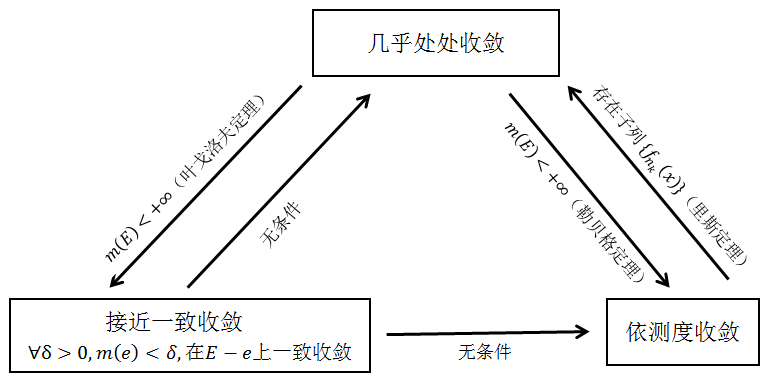
\includegraphics[width=0.8\textwidth]{image/Shoulianxing.png}
\caption{~几种收敛性间的关系} \label{fig33} 
\end{figure}

\section{可测函数与连续函数}

\subsection{卢津定理}

我们知道, 连续函数是可测函数, 可测函数可以由一列简单函数(互不相交闭集上的简单函数是连续函数)来逼近. 本节继续探讨可测函数与连续函数之间更进一步的联系.

\begin{lemma} \label{lem3.1}
设~$F_1,\,\cdots,\,F_n$~为~$\R^n$~中互不相交的闭集, 记~$F = \smallcup\limits_{k=1}^n F_k$, 则简单函数~$f(x) = \sum\limits_{k=1}^n c_k \chi_{F_k} (x)$~是~$F$~上的连续函数.
\end{lemma}

\begin{proof}
设~$x_0 \in F$, 则存在~$k_0$~使得~$x \in F_{k_0}$. 由于~$F_1,\,\cdots,\,F_n$~互不相交, 故~$x \notin \smallcup\limits_{k \neq k_0} F_k$. 又~$\smallcup\limits_{k \neq k_0} F_k$~闭, 则~$d\big(x_0,\,\smallcup\limits_{k \neq k_0} F_k\big) > 0$. 对~$\forall~\varepsilon > 0$, 记~$\delta = d\big(x_0,\,\smallcup\limits_{k \neq k_0} F_k\big)$. 则当~$x \in F$, 且~$d(x,\,x_0) < \delta$~时, 必有~$x \in F_{k_0}$. 从而
\[
|f(x) - f(x_0)| = |c_{k_0} - c_{k_0}| = 0 < \varepsilon
\]
因此, $f(x)$~在点~$x_0$~连续, 由~$x_0$~的任意性, $f(x)$~在~$F$~上连续.
\end{proof}

\begin{theorem}[卢津定理\index{卢津定理}]
设~$f(x)$~为可测集~$E$~上几乎处处有限的可测函数, 则对~$\forall~\delta > 0$, 存在闭集~$F \subset E$, 使得~$m(E - F) < \delta$, 且~$f(x)$~在~$F$~上连续.
\end{theorem}

\begin{proof}
由于~$m\big( \{x \in E: \: |f(x)| = +\infty\} \big) = 0$, 不妨设~$f(x)$~在~$E$~上处处有限.

(1) 若~$f(x)$~为简单函数, 即~$f(x) = \sum\limits_{k=1}^n c_k \chi_{E_k} (x)$, 其中~$E_1, \, \cdots, \, E_n$~可测互不相交且~$\mathop{\cup}\limits_{k=1}^n E_k = E$.

$E_k$~可测, 则对~$\forall~\delta > 0$, 存在闭集~$F_k \subset E_k$, 使得
\[
m(E_k - F_k) < \frac{\delta}{n}, \, \quad k = 1,\,\cdots,\,n
\]
令~$F = \mathop{\cup}\limits_{k=1}^n F_k$, 则~$F$~闭, $F \subset E$, 且
\begin{eqnarray*}
m(E - F) &=& m\big(\medcup\limits_{k=1}^n E_k - \medcup\limits_{k=1}^n F_k \big) = m\big( \medcup\limits_{k=1}^n (E_k - F_k) \big) \\
&\leqslant& \sum_{k=1}^n m(E_k - F_k) < \delta
\end{eqnarray*}
又~$f|_F(x) = \sum\limits_{k=1}^n c_k \chi_{F_k}(x)$, 由引理~\ref{lem3.1}~知~$f|_F$~连续.

(2) 若~$f(x)$~为有界可测函数, 由定理~\ref{thm312}, 存在简单函数列~$\{\varphi_n(x)\}$~在~$E$~上一致收敛于~$f(x)$.

由~(1), 对~$\forall~\delta > 0$~以及每个~$\varphi_n(x)$, 存在闭集~$F_n \subset E$~使得
\[
m(E - F_n) < \frac{\delta}{2^n}
\]
且~$\varphi_n(x)$~在~$F_n$~上连续. 令~$F = \mathop{\cap}\limits_{n=1}^\infty F_n$, 则~$F$~闭, $F \subset E$, 且
\begin{eqnarray*}
m(E - F) &=& m\big( E - \mathop{\cap}_{n=1}^\infty F_n \big) = m\big( \mathop{\cup}_{n=1}^\infty \big(E - F_n\big) \big) \\
&\leqslant& \sum_{n=1}^\infty m(E - F_n) < \sum_{n=1}^\infty \frac{\delta}{2^n} = \delta
\end{eqnarray*}
由于~$\varphi_n(x)$~在~$F$~上连续, 又
\[
\varphi_n(x) \rightrightarrows f(x), \, \quad x \in F \subset E
\]
故~$f(x)$~在~$F$~上连续(连续函数列的一致收敛极限是连续函数).

(3) 若~$f(x)$~为无界可测函数\footnote{可测函数有界与有限的区别: 有界必有限, 但有限不一定有界, 例如~$E=(0,\,1], \, f(x) = 1/x$~在~$E$~上每一点都有限, 但~$f(x)$~在~$E$~上无界.}, 做变换\footnote{``$\Rightarrow$''. $f(x) = g(x) \big( 1 + |f(x)|\big) = \frac{g(x)}{\frac{1}{1 + |f(x)|}} = \frac{g(x)}{1- \frac{|f(x)|}{1 + |f(x)|}} = \frac{g(x)}{1- |g(x)|}$; \\ ``$\Leftarrow$''. $g(x) = f(x)\big(1- |g(x)|\big) = \frac{f(x)}{\frac{1}{1- |g(x)|}} = \frac{f(x)}{1 + \frac{|g(x)|}{1- |g(x)|}} = \frac{f(x)}{1+ |f(x)|}$.}
\[
g(x) = \frac{f(x)}{1+ |f(x)|} \quad \Longleftrightarrow \quad f(x) = \frac{g(x)}{1- |g(x)|}
\]
则~$g(x)$~有界可测, 由~(2), 对~$\forall~\delta > 0$, 存在闭集~$F \subset E$~使得~$m(E - F) < \delta$, 且~$g|_F$~连续. 利用连续函数关于四则运算和~$|\cdot|$~运算封闭, $f(x)$~与~$g(x)$~的连续性
相同, 故~$f|_F$~连续.
\end{proof}

\begin{remark}
(i) 卢津定理说明, 可测函数可以在去掉任意小测度集~$E_\delta$~剩下的集合~$E - E_\delta$~上连续. 换句话说, 可测函数在某个小测度集上改变其函数值, 可以变成连续函数.

(ii) 卢津定理表明可测函数可由连续函数逼近(相差任意小的测度集的方式).

(iii) 定理条件~``~$m(E - F) < \delta$''~不能加强为~``~$m(E - F) = 0$''.
\end{remark}

\begin{example}
考虑狄利克雷函数
\[
D(x) = \left\{ \!\!
\begin{array}{ll}
1, & x \in \Q_{[0,1]} \\[0.1cm]
0, & x \in [0,\,1]-\Q_{[0,1]}
\end{array}
\right.
\]
记~$\Q_{[0,1]} = \{r_n\}_{n=1}^\infty$, 对~$\forall~\delta > 0$, 令
\[
F_\delta = [0,\,1] - \medcup_{n=1}^\infty \Big( r_n - \frac{\delta}{2^{n+1}},\, r_n + \frac{\delta}{2^{n+1}} \Big)
\]
则~$F_\delta$~闭, 且
\[
m\big([0,\,1] - F_\delta \big) = m \Big( \medcup_{n=1}^\infty \Big( r_n - \frac{\delta}{2^{n+1}},\, r_n + \frac{\delta}{2^{n+1}} \Big) \Big) \leqslant \sum_{n=1}^\infty \frac{\delta}{2^n} = \delta
\]
而~$D(x)$~在~$F_\delta$~上恒等于~$0$, 从而~$D(x)$~在~$F_\delta$~上是连续的.
\end{example}

\begin{theorem}[卢津定理的逆定理\index{卢津定理的逆定理}, 可测函数的又一定义]
设~$f(x)$~为可测集~$E$~上几乎处处有限的实值函数, 若对~$\forall~\delta > 0$, 存在闭集~$F_\delta \subset E$, 使得~$m(E - F_\delta) < \delta$, 且~$f(x)$~在~$F_\delta$~上连续, 则~$f(x)$~是~$E$~上的可测函数.
\end{theorem}

\begin{proof}
对每个~$n \in \N$, 都存在闭集~$F_n \subset E$~使得~$m(E - F_n) < 1/n$, 且~$f(x)$~在~$F_n$~上连续, 故~$f(x)$~在~$F_n$~上可测.

记~$F = \mathop{\cup}\limits_{n=1}^\infty F_n$, 则~$f(x)$~在~$F$~上可测. 由于~$F_n \subset F, \, n = 1,\,2,\,\cdots$, 故
\[
m(E - F) \leqslant m(E - F_n) < \frac{1}{n}, \, \quad n = 1,\,2,\,\cdots
\]
令~$n \to \infty$~得, $m(E - F) = 0$. 从而~$f(x)$~在~$E - F$~上可测. 因此, $f(x)$~在~$E = F \cup (E - F)$~上可测.
\end{proof}

\begin{theorem}[卢津定理的另一种形式\index{卢津定理的另一种形式}] \label{thm333}
设~$f(x)$~为可测集~$E$~上几乎处处有限的可测函数, 则对~$\forall~\delta > 0$, 都存在~$\R^n$~上的连续函数~$g(x)$~使得
\[
m\big(\{x \in E: \: f(x) \neq g(x)\} \big) < \delta
\]
且~$\sup\limits_{x \in \R^n} |g(x)| \leqslant \sup\limits_{x \in E} |f(x)|$. 若~$E$~是有界集, 则可要求~$g(x)$~具有紧支集\footnote{集合~$\{x \in D(f): \: f(x) \neq 0\}$~称为函数~$f$~的支撑集, 记为~$\mathrm{supp~}\!(f)$. 若~$\mathrm{supp~}\!(f)$~是紧集, 则称函数~$f$~具有紧支集. }.
\end{theorem}

\begin{proof}
由卢津定理, 对~$\forall~\delta > 0$, 存在闭集~$F \subset E$~使得~$m(E - F) < \delta$, 且~$f(x)$~在~$F$~上连续. 由连续函数延拓定理~\ref{thm1414}, 存在~$\R^n$~上的连续函数~$g(x)$~使得
\[
g(x) = f(x), \, \quad x \in F
\]
且~$\sup\limits_{x \in \R^n} |g(x)| \leqslant \sup\limits_{x \in E} |f(x)|$.
由于
\[
\{x \in E: \: f(x) \neq g(x)\} \subset E - F
\]
故
\[
m\big(\{x \in E: \: f(x) \neq g(x)\} \big) \leqslant m(E - F) < \delta
\]

若~$E$~有界, 不妨设~$E \subset B(0,\,r)$. 作~$\R^n$~上的连续函数~$\varphi(x)$, 满足~$0 \leqslant \varphi(x) \leqslant 1$, 且
\[
\varphi(x) = \left\{\!\!
\begin{array}{ll}
1, & x \in E \\[0.1cm]
0, & x \notin B(0,\,r)
\end{array}
\right.
\]
则把~$g(x)$~换成~$\varphi(x)g(x)$~即为所求.
\end{proof}

\begin{theorem}
设~$f(x)$~为可测集~$E$~上几乎处处有限的可测函数, 则存在~$E$~上的连续函数列~$\{f_n(x)\}$~
使得~$f_n \xrightarrow{\mathrm{a.e.}} f$.
\end{theorem}

\begin{proof}
由定理~\ref{thm333}, 对每个~$n \in \N$, 都存在~$\R^n$~上的连续函数~$g_n(x)$~满足
\[
m\big(\{x \in E: \: f(x) \neq g_n(x)\} \big) < \frac{1}{n}
\]
从而, 对~$\forall~\varepsilon > 0$
\begin{eqnarray*}
&& m\big( \{x \in E: \: |g_n(x) - f(x)| \geqslant \varepsilon \} \big) \\
&\leqslant& m\big(\{x \in E: \: f(x) \neq g_n(x)\} \big) < \frac{1}{n} \longrightarrow 0
\end{eqnarray*}
当~$n \to \infty$~时. 故~$g_n \xrightarrow{~\mu~} f$. 由里斯定理, 存在~$\{g_n\}$~的子列~$\{g_{n_k}\}$~
使得~$g_{n_k} \xrightarrow{\mathrm{a.e.}} f$. 再取~$f_k = g_{n_k}|_E$~即可.
\end{proof}

\section{测度论与概率论的关系$^\ast$}

测度论是概率论的理论基础, 所以, 概率论中的一些概念抽象化就是对应的测度论中的概念. 

概率是要度量``事件发生的可能性''的大小, 事件的抽象化描述就是集合, 需要考察``事件的全体'', 对应到测度论就是``集合系''. ``事件发生的可能性''是对事件的一种度量, 对应到测度论就是``集合的测度''. 

不是每个事件都可以定义其概率（发生的可能性的大小）的, 对应的就是不是每个集合都可以定义测度, 可以定义测度集合就是可测集. 同时, 事件必然要涉及到事件的组合运算（复杂事件是可由基本事件表示出来）, 对应的就是集合的交、并、差、余、极限的运算到复杂集合, 所以又需要保证做可列次这些运算不能超出全体范围（即可测集的范围要足够大, 以保证集合的可列次交、并、差、余、极限等的运算之后还在里面）.

那么什么样的集合系, 才能保证其中的集合是可测集（可以定义测度，又对那些运算封闭）呢? 测度论中讲了, 只要集合系是~$\sigma$-代数就可以了。$\sigma$-代数的基本定义是: 

\begin{publist}
	\item[(1)] 全集在里面; 
	
	\item[(2)] 里面每个集合的余集在里面; 
	
	\item[(3)] 里面任意可列个集合的并集在里面.
\end{publist}

\noindent 有了这三条基本定义, 就可以推出: 空集、可列次交、并、差、上限集、下限集等运算之后都能在里面, 就满足需要了.

所以, 集合~$X$, 再加上该集合上的一个~$\sigma$-代数~$\F$, $(X, \F)$~就是一个可测空间了, 即可以定义测度的空间, $\F$~中任一集合都可以定义其测度（集合大小的某种度量）. 进一步再定义了测度~$\mu$, 那么~$(X,\F,\mu)$~就是测度空间.

对应到概率论中, 样本空间（集合）~$\Omega$, 事件域~$\F$（$\sigma$-代数），概率测度~$P$（测度）, 放一起~$(\Omega,\F,P)$~就是概率测度空间, 简称概率空间. 概率测度~$P$~是满足特殊要求的一种测度: $P(\Omega)=1$.

Borel~$\sigma$-代数~$\mathfrak{B}_\R$, 表示实数轴~$\R$~上的~$\sigma$-代数, 可由实轴上的所有开集生成, 也可由实数轴上所有的~$(-\infty,a]$~这样的区间生成, 是相等的. 按~$\sigma$-代数定义, 实数轴上开集、闭集的至多可列次交、并、差（余）、上限集、下限集、极限集的运算, 都超不出该~Borel~$\sigma$-代数的范围.

$\mathfrak{B}_\R$~有什么用? 其实概率论中的随机变量, 对应测度论中的可测函数, 而可测函数就是从可测空间~$(X,\F)$~到~$(\R, \mathfrak{B}_\R)$~的可测映射: 即~$\mathfrak{B}_\R$~中的任一集合在该映射下的原像都属于~$\F$（即都是~$X$~上的可测集）.

再说说随机变量, 前面说了概率论中要用集合表示事件, 但事件五花八门, 怎么统一用一种简单的集合表示呢? 这就用到映射的概念, 建立一种从样本空间（基本事件的全体）到实数轴的映射（一一对应）就可以了, 这种映射就是随机变量. 有了它，基本事件映射到实数轴上就是的基本区间, 基本事件经过运算生成的复杂事件, 映射到实数轴上就是~$\mathfrak{B}_\R$中的集合, 即~Borel~集. 

因为有了这个对应关系, 要度量``事件发生的可能性的大小''（即概率测度）, 只要度量``实数轴上~Borel~$\sigma$-代数中的集合'' 就可以了. 而~$\mathfrak{B}_\R$~是~$\sigma$-代数是可以定义测度的, 于是给~$\mathfrak{B}_\R$~中的集合定义概率测度就行了.

所以, 随机变量的测度论语言定义是这样的: 设~$(\Omega,\F,P)$~为概率空间，若对实数轴上~$\sigma$-代数~$\mathfrak{B}_\R$~中的任一集合~$B$, 都有~$\{ \omega \in \Omega: X(\omega) \in B\} \in \F$, 则称~$X(\omega)$~为随机变量, 也简记为~$X$.

总之, 随机变量就是建立了``随机事件''到``实数轴上~Borel~$\sigma$-代数''的一种对应, 并且保证了建立了这种对应的随机事件都是可以定义概率测度的. 

既然随机事件~$\{\omega \in \Omega: X(\omega) \in B\}$~属于~$\F$, 那么可以有概率, 即~$P\{\omega \in \Omega: X(\omega) \in B\}$~是有意义的. 为了简单, 概率中简记
\[
P\{\omega \in \Omega: X(\omega) \in B\} = P\{X \in B\}
\] 

特别地, 若取~$B=(-\infty,x)$, 则事件~$\{X \in B\}$~的概率
\[
P\{X \in B\} = P\{X \leqslant x\} := F(x)
\]
就定义成随机变量~$X$~的分布函数. 因为对任意的区间~$(a,b]$, 都可表示成
\[
P\{X \in (a,b] \} = P\{a < X \leqslant b\} = P\{X \leqslant b\} - P\{X \leqslant a\} = F(b)-F(a)
\]
进而, 由这样的区间经过至多可列次交、并、差运算的复杂的实数轴上的~Borel~集都可以用~$F(x)$~给出其概率.

当然, 随机变量也可以定义为从样本空间到平面~$\R^2$~上的映射, 就是二元随机变量.

\newpage
\begin{problemset}

\item $f$~可测~$\Leftrightarrow$~对~$\forall~r \in \Q$, $\{x \in E: \: f(x) > r\}$~是可测集. 若~``~$f(x) > r$~''~换成~``~$f(x) = r$~'', 结论不成立.

\item 设~$f(x)$~是~$E$~上的可测函数, $G,\,F$~分别为~$\R$~中的开集和闭集, 问
    \[
    \{x \in E: \: f(x) \in G\}, \quad \{x \in E: \: f(x) \in F\}
    \]
    是否是可测集? 下列结论是否成立?

\begin{enumerate}
  \item[(1)] $f$~可测~$\Leftrightarrow$~对任意的开集~$G \subset \R$, $\{x \in E: \: f(x) \in G\}$~是可测集.
  \item[(2)] $f$~可测~$\Leftrightarrow$~对任意的闭集~$F \subset \R$, $\{x \in E: \: f(x) \in F\}$~是可测集.
\end{enumerate}

\item 从函数~$f^2(x)$~或~$|f(x)|$~可测, 能否推出~$f(x)$~也可测?

\item 由~$f(x)\pm g(x)$~可测, 能否推出~$f(x),\,g(x)$~都可测?

\item 设~$\{f_n(x)\}$~为~$E$~上的可测函数列, 能否断定~$\sum\limits_{n=1}^\infty f_n(x)$~为~$E$~上的可测函数?

\item 设~$E$~是~$[0,\,1]$~中的不可测集
\[
f(x) = \left\{\!\!
\begin{array}{cl}
x, \, & x \in E \\[0.1cm]
-x, \, & x \in [0,\,1] - E
\end{array}
\right.
\]
问~$f(x)$~在~$[0,\,1]$~上是否可测? $|f(x)|$~是否可测?

\item 设~$\{f_n(x)\}$~为~$E$~上的可测函数列, 则其收敛点集与发散点集都是可测的.

\item 试证如下的黎曼函数是可测函数
\[
R(x) = \left\{\!\!
\begin{array}{cl}
\dfrac{1}{n}, \, &  x = \dfrac{m}{n} \\[0.2cm]
0, \, &  x \mbox{~为无理数}
\end{array}
\right.
\]
(其中, $x \in [0,\,1],\,m,\,n$~互质, 且~$m \leqslant n$).

\item 设~$f(x)$~为~$E$~上几乎处处有限的可测函数, $m(E) < +\infty$, 则对~$\forall~\varepsilon > 0$, 都存在有界可测函数~$g(x)$~使得
\[
m\big( \{x \in E:\: f(x) \neq g(x) \}\big) < \varepsilon
\]

\item 设~$f(x)$~为~$E$~上的可测函数, $g(x)$~为~$\R$~上的波雷尔可测函数, 试证 $g(f)$~是~$E$~上的可测函数.

\item 设~$f(x)$~为~$[a,\,b]$~上的可微函数, 则~$f'(x)$~在~$[a,\,b]$~上可测.

\item 设在可测集~$E$~上有~$f_n \xrightarrow{\mathrm{a.e.}} f, \, g_n \xrightarrow{\mathrm{a.e.}} g$. 证明:

\begin{enumerate}
  \item[(1)] $a f_n + b g_n \xrightarrow{\mathrm{a.e.}} a f + b g, \, \forall~a,\,b \in \R$;
  \item[(2)] $|f_n| \xrightarrow{\mathrm{a.e.}} |f|$;
  \item[(3)] $\sup\{f_n,\,g_n\} \xrightarrow{\mathrm{a.e.}} \sup\{f,\,g\}$; $\inf\{f_n,\,g_n\} \xrightarrow{\mathrm{a.e.}} \inf\{f,\,g\}$.
\end{enumerate}

\item 设在可测集~$E$~上有~$f_n \xrightarrow{~\mu~} f, \, g_n \xrightarrow{~\mu~} g$. 证明:

\begin{enumerate}
  \item[(1)] $a f_n + b g_n \xrightarrow{~\mu~} a f + b g, \, \forall~a,\,b \in \R$;
  \item[(2)] $|f_n| \xrightarrow{~\mu~} |f|$;
  \item[(3)] $\sup\{f_n,\,g_n\} \xrightarrow{~\mu~} \sup\{f,\,g\}$; $\inf\{f_n,\,g_n\} \xrightarrow{~\mu~} \inf\{f,\,g\}$.
\end{enumerate}

\item 设~$m(E) > 0$, $\{f_n(x)\}$~为~$E$~上几乎处处有限的可测函数列, 且~$f_n \xrightarrow{\mathrm{a.e.}} f$, 则存在常数~$C$~与~$E_0 \subset E$, 满足~$m(E_0) > 0$, 且
    \[
    |f_n(x)| \leqslant C, \, \quad \forall~x \in E_0, \, n \in \N
    \]

\item 设~$m(E) < +\infty$, 对于在~$E$~中每点都趋于~$+\infty$~的函数列建立叶戈洛夫定理.

\item 问当~$m(E)=+\infty$~时, 卢津定理是否仍然成立?

\item 试作~$E = [0,\,1]$~上的可测函数~$f(x)$, 使得对~$E$~上任意连续函数~$g(x)$~都有
    \[
    m\big(\{x \in E: \: f(x) \neq g(x)\} \big) \neq 0
    \]
    此结果与卢津定理有无矛盾?

\item 设对每个给定的~$n$, 当~$k \to \infty$~时, $f_k^{(n)}(x) \xrightarrow{~\mu~} f^{(n)}(x)$, 且当~$n \to \infty$~时, $f^{(n)}(x) \xrightarrow{~\mu~} f(x)$. 则在~$\big\{ f_k^{(n)}(x) \big\}$~中可以选取函数列依测度收敛于~$f(x)$.

\item 设~$f_n \xrightarrow{~\mu~} f$, 且对每个~$n \in \N$~都有~$f_n(x) \leqslant g(x)$. 证明~$f(x) \leqslant g(x), \, \mathrm{~a.e.~} x \in E$.

\item 设~$f_n \xrightarrow{~\mu~} f$, 且对每个~$n \in \N$~都有~$f_n(x) \leqslant f_{n+1}(x), \, \mathrm{~a.e.~} x \in E$. 证明~$f_n \xrightarrow{\mathrm{a.e.}} f$.

\item 设~$f(x),\,f_1(x),\,\cdots,\, f_k(x),\,\cdots$~为~$E=[a,\,b]$~上几乎处处有限的可测函数, 且在~$E$~上有~$f_k \xrightarrow{\mathrm{a.e.}} f$. 则存在可测集~$E_n \subset [a,\,b]$, $n=1,\,2,\,\cdots$, 使得
    \[
    m\Big( [a,\,b]-\medcup_{n=1}^\infty E_n \Big) = 0
    \]
    而在每个~$E_n$~上有~$f_k \rightrightarrows f$.

\item 设~$f(x)$~为~$[a,\,b]$~上的几乎处处有限的可测函数, 则对任意的~$\varepsilon > 0$~及~$\delta > 0$, 都存在闭集~$F \subset [a,\,b]$~及多项式函数~$P(x)$, 使得~$m(F) > b-a-\delta$, 且
    \[
    \big| f(x) - P(x) \big| < \varepsilon, \quad x \in F
    \]

\item 设~$f(x)$~为~$[a,\,b]$~上的实值可测函数, 证明: 存在数列~$\{h_n\}$, 使得
    \[
    \lim_{n \to \infty} h_n = 0, \, \quad \lim_{n \to \infty} f(x+h_n) = f(x), \quad \mathrm{~a.e.~} x \in [a,\,b]
    \]

\item 设~$\{f_n(x)\}$~为~$[0,\,1]$~上几乎处处收敛于~$0$~的可测函数列, 证明: 存在数列~$\{t_n\}$, 使得
\[
\sum_{n=1}^\infty |t_n| = +\infty, \, \quad \sum_{n=1}^\infty \big| t_n f_n(x) \big| < +\infty, \quad \mathrm{~a.e.~} x \in [0,\, 1]
\]
\end{problemset}


